\documentclass[border=10pt]{standalone}

\usepackage{tikz}
\usepackage{tikzsymbols}
\usetikzlibrary{calc,patterns,shapes.geometric}

\def\centerarc[#1](#2)(#3:#4:#5){\draw[#1] ($(#2)+({#5*cos(#3)},{#5*sin(#3)})$) arc (#3:#4:#5);}

\begin{document}
	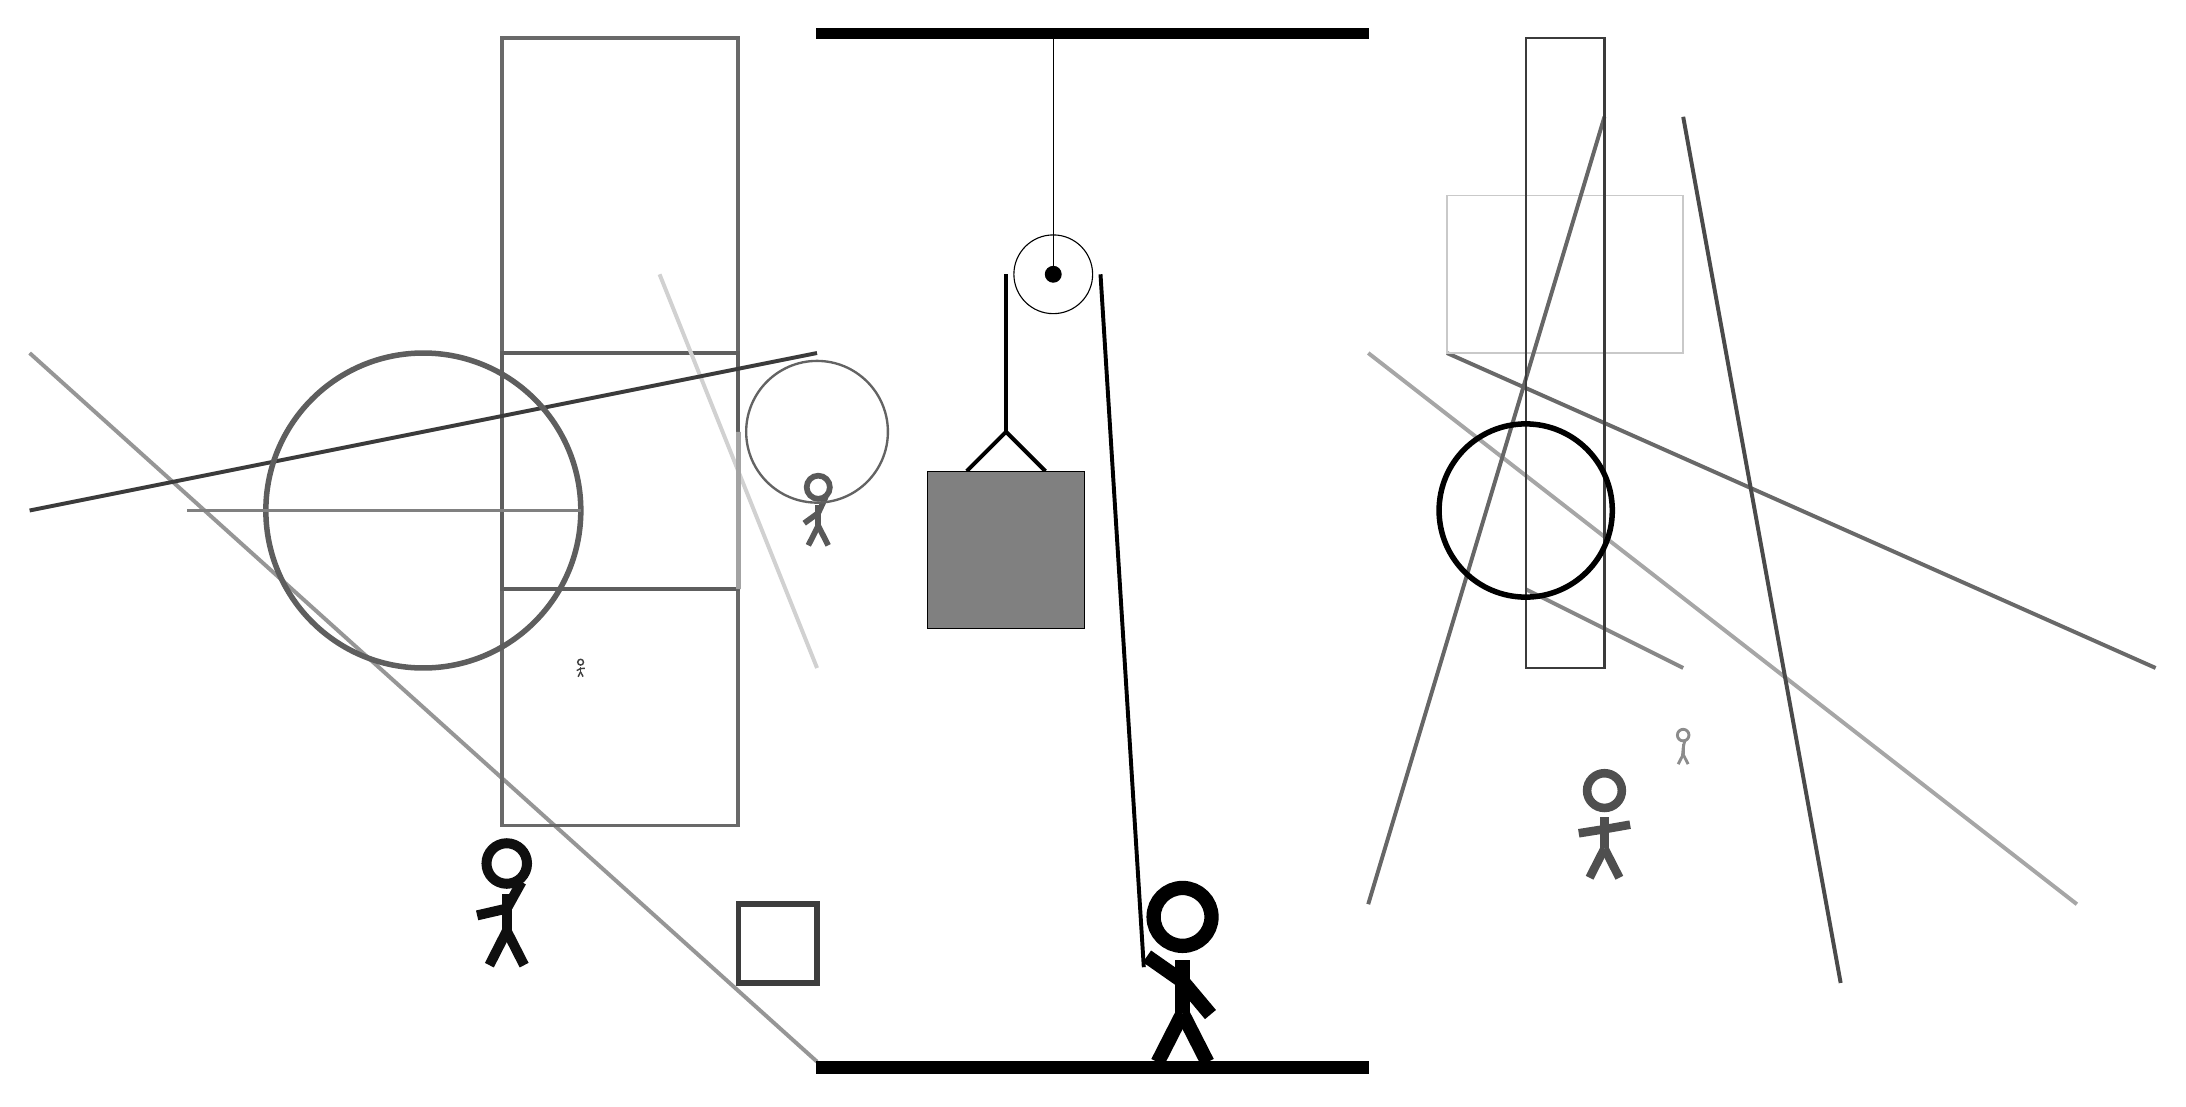
\begin{tikzpicture}
		%%%%% START %%%%%
		
		\draw[fill=black] (-2, 10) rectangle (5, 10.125);
		
		\draw (1, 7) circle (0.5);
		\draw[fill=black] (1, 7) circle (0.1);
		\draw (1, 10) -- (1, 7);
		
		\draw[line width=0.5mm, color=black!41](-2, -3) -- (-12, 6);
		
		\draw[line width=0.5mm, color=black!59] (-3, 10) rectangle (-6, 0);
		\draw[line width=0.5mm, color=black!59](6, 6) -- (15, 2);
		\node[line width=0.3mm, color=black!75] at (-5, 2) {\Strichmaxerl[1][27][4]};
		\node[line width=0.3mm, color=black!69] at (8, 0) {\Strichmaxerl[6][9][10]};
		
		\draw[line width=0.5mm, color=black!35](5, 6) -- (14, -1);
		\draw[line width=0.5mm, color=black!63] (-3, 6) rectangle (-6, 3);
		
		\node[line width=0.6mm, color=black!65] at (-2, 4) {\Strichmaxerl[4][36][65]};
		\draw[line width=0.5mm, color=black!18](-4, 7) -- (-2, 2);
		\node[line width=0.2mm, color=black!45] at (9, 1) {\Strichmaxerl[2][85][78]};
		
		\draw[line width=0.2mm, color=black!21] (6, 8) rectangle (9, 6);
		
		\draw[line width=0.7mm, color=black!76] (-3, -1) rectangle (-2, -2);
		\draw[line width=0.5mm, color=black!77](-2, 6) -- (-12, 4);
		
		\node[line width=0.7mm, color=black!94] at (-6, -1) {\Strichmaxerl[7][13][61]};
		\draw[line width=0.5mm, color=black!60](8, 9) -- (5, -1);
		\draw [line width=0.7mm, color=black!63](-7, 4) circle (2.0);
		\draw [line width=0.3mm, color=black!61](-2, 5) circle (0.9);
		\draw[line width=0.5mm, color=black!47](7, 3) -- (9, 2);
		\draw[line width=0.5mm, color=black!50](-5, 4) -- (-10, 4);
		
		\draw[line width=0.3mm, color=black!77] (7, 2) rectangle (8, 10);
		\draw[line width=0.5mm, color=black!71](9, 9) -- (11, -2);
		\draw[line width=0.6mm, color=black!36] (-3, 5) rectangle (-3, 3);
		\draw [line width=0.7mm, color=black!100](7, 4) circle (1.1);
		
		\draw[line width=0.5mm] (-0.1, 4.5) -- (0.4, 5.0) -- (0.9, 4.5);
		\draw[fill=black!50] (-0.6, 4.5) rectangle (1.4, 2.5);
		
		\draw[line width=0.5mm] (0.4, 7) -- (0.4, 5.0);
		\centerarc[line width=0.5mm](1, 7)(0:180:0.6);
		\draw[line width=0.5mm](1.6, 7) -- (2.15, -1.8);
		
		\node at (2.6, -1.9) {\Strichmaxerl[10][-35][-50]};
		
		\draw[fill=black] (-2, -3) rectangle (5, -3.15);
		
		%%%%% END %%%%%
	\end{tikzpicture}
\end{document}